\thispagestyle{endchapter}

\begin{tcolorbox}
\vspace{80pt}

\lettrine{I}{n} all, 2.2km of new cave was found during the 2010 Vodna Sled expedition, taking \passage{Vrtnarija} to 8.776 km. We are in the extremely fortuitous circumstance where we finish the year with considerably more leads in the \passage{Migovec} cave systems
than we started with. The \passage{X-ray} camp was derigged with the certainty that we will be back next year camping in the same location. Gas cylinders and cans of fish were left sealed in Daren drums with
a rock of carbide to keep them dry, the carry mats and tents were left standing to air, and we have a considerable armoury of rope brought back from the pushing fronts waiting for the 2011 team.

The work by the JSPDT in the Autumn has ‘opened up‘ \passage{M2} once again and brought the possibility of forging a connection back to the table. The pushing of the \passage{Republica} streamway (now \passage{Insomnia}) to within
a few metres of the maximum depth of the cave has reawakened the possibility of further depth extension to \passage{Vrtnarija}. Expedition members have mooted the possibility of establishing an additional 2-man
‘deep camp’ to benefit pushing trips in the lower reaches of the cave, particularly any revisits to the far North end of the system.

The significant discoveries of this year have been the fruit of the communal effort of ICCC and JSPDT members. When System \passage{Vrtnarija} and \passage{System Mig} will be connected, the cave will only be 500m shorter than the
\passage{Postonjska Jama} system. Suddenly the plain dwellers will have to rewrite their tourist brochures and the thought of the longest cave in Slovenia will not be a dream. Oh, and the cave has the potential to be 1km
deep (requiring an additional 120m of depth from \passage{Insomnia}).

As well as being proud of each metre of survey we should also think about each metre that a tackle sack was carried, each meal cooked, each bottle of booze safely ferried to camp. A significant factor in our success is evident because it needs not mentioning: thanks to efficient and thoughtful organization we did not run out of any goods, the stereo batteries were always full, the food supplies always high. And most importantly, we have no accidents to report.

\end{tcolorbox}
	\backgroundsetup{	scale=1.1,
        color=black,
        opacity=1,
        angle=0,
        contents={%
                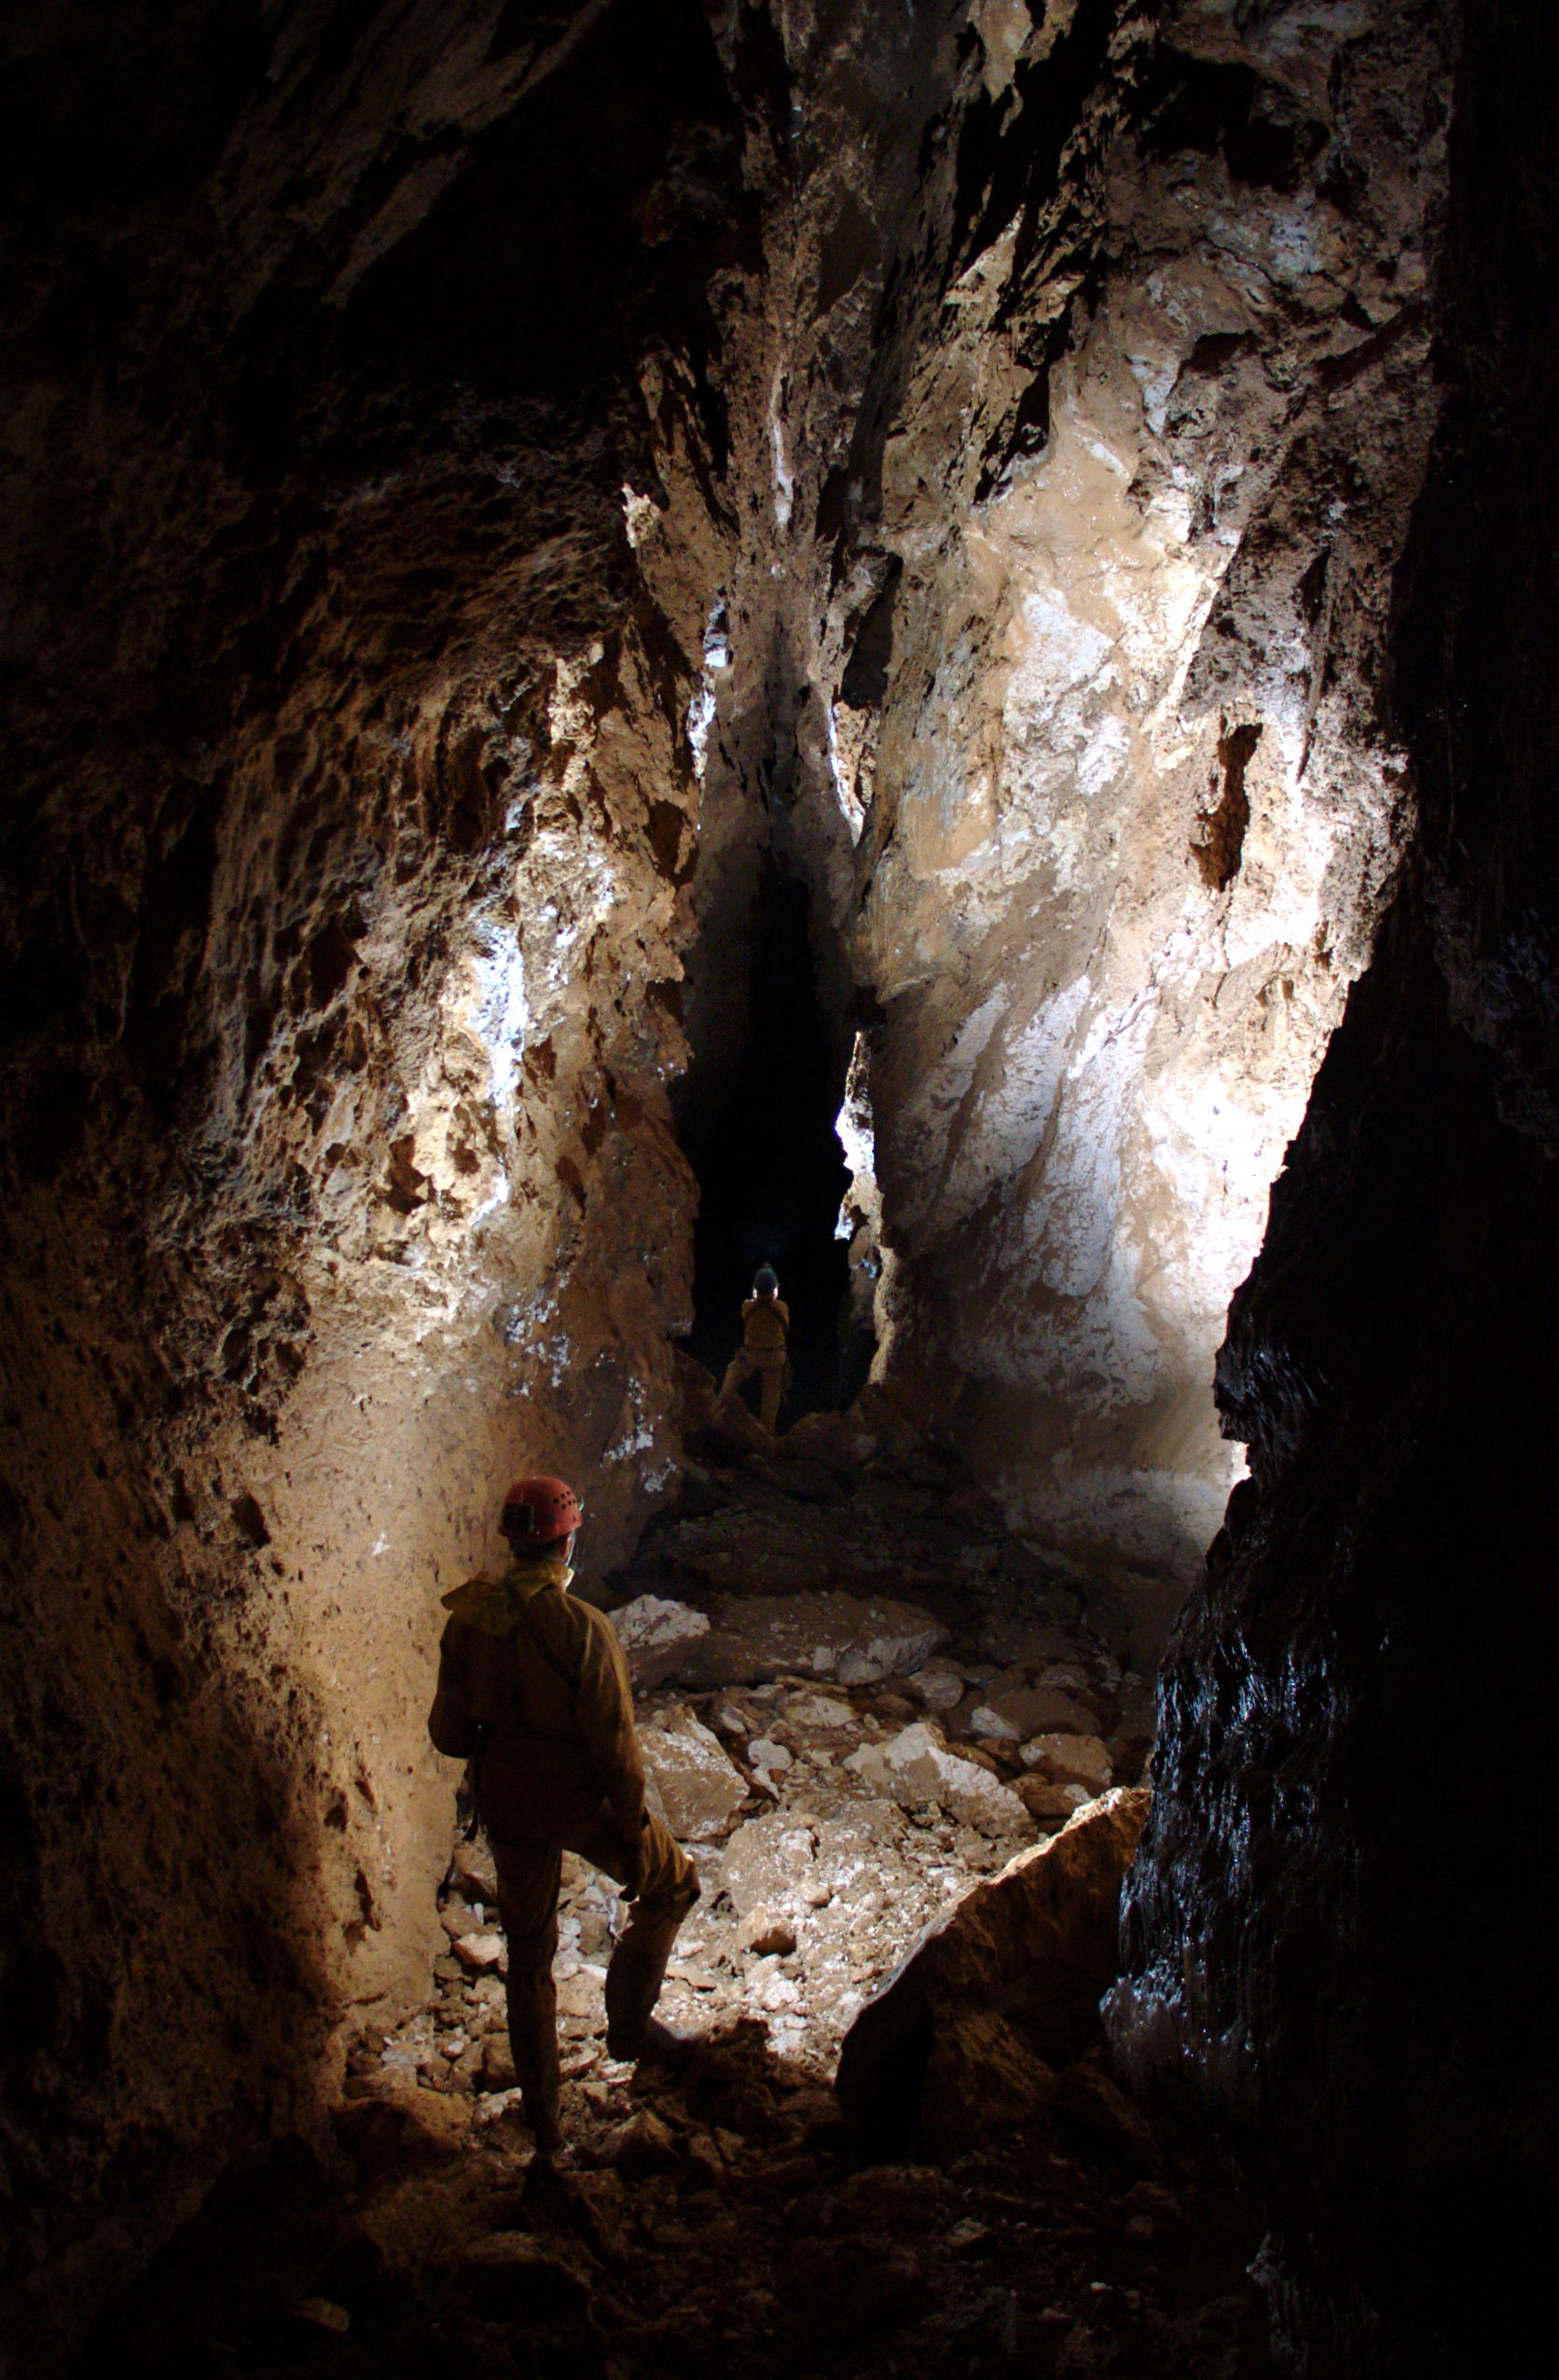
\includegraphics[height=\paperheight]{2010/outro/20100731-19-59-40-Jarvist Frost-Canon G5-CRW_0351-straightened_cropped-Further Down Minotaur Rift - Palace of King Minos--orig.jpg}
        }
	}
\BgThispage
